\documentclass[12pt,a4paper]{report}
%\fontencoding{T1}

\usepackage[utf8]{inputenc}
\usepackage[T1]{fontenc}
\usepackage[danish]{babel}
\usepackage[hidelinks]{hyperref}
\usepackage{lingmacros}
\usepackage{tree-dvips}
\usepackage{url}
\usepackage{array}
\usepackage{graphicx}
\usepackage{float}
\usepackage{lastpage}
\usepackage{color}
\usepackage[x11names,rgb,usenames,dvipsnames,svgnames,table]{xcolor}
\usepackage{colortbl}
\usepackage{algorithm2e}
\usepackage{geometry}
\usepackage{titlesec, blindtext, color}
\definecolor{gray75}{gray}{0.75}
\definecolor{gray90}{gray}{0.90}
\definecolor{ForestGreen}{RGB}{15,116,61}
\definecolor{gray25}{gray}{0.25}
\newcommand{\hsp}{\hspace{20pt}}

\usepackage{tikz}
\usetikzlibrary{snakes,arrows,shapes}
\usepackage{amsmath}

\usepackage{xcolor} 
\usepackage{fix-cm} 
\usepackage{pgfplots}

%Titelblad fix
%\usepackage[ansinew]{inputenc}
\usepackage{a4}

\titleformat{\chapter}[hang]{\Huge\bfseries}{\thechapter\hsp\textcolor{gray75}{|}\hsp}{0pt}{\Huge\bfseries}

\begin{document}
\setcounter{page}{2}

\begin{titlepage}
\newcommand{\HRule}[1]{\hfill \rule{0.2\linewidth}{#1}} 

\definecolor{grey}{rgb}{0.9,0.9,0.9} 
\newgeometry{top=2in,bottom=1in,right=0cm,left=0cm}
\thispagestyle{empty} 

\noindent \colorbox{grey}{
	 \parbox[t]{1.0\linewidth}{
		\centering \fontsize{50pt}{80pt}\selectfont
		\vspace*{0.7cm}
		P1-Rapport \\[3pt]
        \LARGE Komprimering af korte beskeder \\ 
		\vspace*{0.7cm}
	}
}

\vfill
\flushright
\flushright \rule[10pt]{0.1pt}{160pt}  \begin{minipage}[b]{0.45\linewidth}
{
\Large
\textbf{Gruppe B228:} \\[4pt]
Bossen, Jannek Alexander Westerhof\\[.2cm]
Brämer, Kevin\\[.2cm]
Bønneland, Frederik Meyer\\[.2cm]
Joensen, Ólavur Debes\\[.2cm]
Olesen, Anders Trier\\[.2cm]
Tjell, Katrine Sofie\\[.2cm]
}
\end{minipage}

\clearpage 

%\title{P1-Rapport}
%\author{B228}
%\date{\today}
%\pagebreak
%\maketitle
%% Fjerner sidetal på forsiden
\thispagestyle{empty}
\end{titlepage}


\tableofcontents
% Fjerner sidetal på indholdsfortegnelse
\thispagestyle{empty}

\renewcommand{\chaptername}{Kapitel}

% TEKST SÆTTES UNDER HER
\chapter{Indledning}
\setcounter{page}{3}
	Denne analyse har til formål at dokumentere P1 projektforløbet for gruppe B128. Derudover er formålet at reflektere over samarbejdet og arbejdsgangen i gruppen.
\\
Gruppen består af de samme personer som i P0-projektet og i P0-projektforløbet, gik samarbejdet godt og vi fungerede fint sammen socialt. Derfor blev det besluttet at fortsætte i P1 i samme gruppe, og vi valgte så et emne, som vi alle synes var spændende. Derved kendte vi alle hinanden og det gjorde at det var let at komme i gang med projektet, da vi ikke skulle bruge tid på at lære hinanden at kende. Vi havde i gruppen en forventning om at projektet skulle forløbe nogenlunde som det havde gjort i P0. Derudover havde alle en forventning om at ambitionsniveauet skulle være højt og projektet skulle ende med at ligge over middel. 
\\
Med hensyn til udbyttet af projektet, havde vi en forventning om, at lære mere om at skrive en god rapport, og at få gruppearbejdet til at køre. Derudover havde vi også bestemt os for at alle i gruppen skulle lære at bruge \LaTeX{} og ligeledes skulle vi lære at bruge GitHub i stedet for Dropbox, som blev brugt i P0.  
 %Indhold af Indledning.tex bliver sat ind her.
	

\chapter{Projektplanlægning og projektstyring}
 
    \section{Beskrivelse}
Vi har tidligt i projektet udarbejdet en tidsplan over hele projektperioden, hvori vi lavede deadlines for hvornår de forskellige ting i projektet skulle være færdiggjort, se bilag. Vi har dog ikke været særlig gode til at benytte os af planen og vi har heller ikke holdt den opdateret. I stedet har vi delt opgaver ud fra dag til dag og aftalt tidspunkter for hvornår opgaverne skulle være færdiggjort. Ved vores daglige arbejde i grupperummet opgjorde vi status af projektet og aftalte ting som hvornår vi skulle mødes næste dag. 

I P0-projektet, brugte vi Dropbox til fildeling. Det blev lidt besværligt, at hvis 2 personer havde den samme fil åben på engang, blev der skabt en conflicted copy. Derfor valgt vi denne gang at bruge GitHub til at dele filer mellem os og det virkede rigtig godt. Vi brugte dog noget tid i starten af projektet på at få det til at fungere, men det var tid der var godt givet ud. 

Vi valgte fra starten af projektet, at vi ikke skulle have en projektleder. Der var altså ikke én person der havde styringen, derimod havde alle ansvar for at holde arbejdet i gang og vi skiftedes til at være motivator, når der var brug for det. Der blev heller ikke delt andre grupperoller ud.  

Midt i projektforløbet, blev der afholdt statusseminar. Her fik vi gode idéer og forslag til rettelser fra både vejledere og opponentgruppe. Til seminaret valgte vi at 4 ud af gruppens 7 medlemmer skulle fremlægge, hvorefter alle 7 selvfølgelig deltog i diskussionen. Efter statusseminaret rettede vi selvfølgelig det, som vi havde fundet ud af ikke var godt nok, og derefter havde vi faktisk lidt svært ved at komme videre. På GitHub.com kan man se en graf over hvor meget aktivitet der har været i projektet i forhold til tiden. Her fremgår det tydeligt at, vi kom lidt langsomt fra start og lavet rigtig meget kort forinden statusseminaret. Efter seminaret stod det igen lidt stille og først lige op til aflevering af projektet har vi lavet meget igen. 

\section{Analyse}

\emph{Gode erfaringer:}
\begin {itemize}
\item  GitHub var et rigtig godt alternativ til Dropbox – det vil vi klart benytte i fremtidige projekter.

\item	At aftale mødetidspunkt for dag til dag – når folk ellers mødte til tiden. 

\item	Statusseminaret var rigtig godt til at øve en fremlæggelse af det foreløbige projekt og til at få nye ideer.

\item	LaTex er et rigtig godt program til at skrive rapport i.
\end{itemize}\emph{Dårlige erfaringer:}
\begin{itemize}
\item	Vi arbejdede først igennem lige optil en deadline (statusseminar eller endelig aflevering). Det havde været bedre med en konstant arbejdsindsats. 

\item	Ikke at have en ordentlig tidsplan, som blev opdateret, gjorde at vi indimellem mistede overblikket over projeket. 

\item	At tilføje noget til rapporten uden det er ordentlig læst igennem, af mindst to personer.

\item	Man kunne vælge én person, som skulle tage sig af praktiske ting, som kontakt med vejleder, opdatere tidsplan osv. Man kunne skiftes til at have rollen hver uge eksempelvis. 
\end{itemize}

\section{Forbedringer til P2}

I næste projekt skal vi forbedre brugen af en struktureret plan over projektet, så vi undgår at miste overblikket, som det ind imellem er sket i denne projektperiode. Derudover skal vi fra starten uddele ansvaret for de forskellige dele af projektet mellem alle mand, så vi er sikre på at alt bliver lavet. Der skal også være mere fokus på tidsplanen gennem projektet, så der kommer flere deldeadlines. På den måde kan vi måske undgå at arbejdsindsatsen bliver så ”bølget”, og vi kan undgå at der kommer som en overraskelse at der eksempelvis kun er 2 uger til afleveringer.

Det ville nok også være en god ide at have en eller anden form for rollefordeling. En projektleder, sekretær og lignende. Man kunne bytte hver uge for at alle kunne prøve at have de forskellige roller. Måske kunne projektet på den måde blive mere struktureret.



\chapter{Samarbejde i gruppen}
 
    \section{Beskrivelse}
I starten af projektet skrev vi en gruppekontrakt. Vi skrev den mest for at prøve det og derved øve os i at udarbejde en skriftlig aftale. Vi synes den var lidt svær at lave, fordi gruppen i P0 projektet ikke havde haft konflikter eller andre problemer, som man kunne have beskrevet hvordan de skulle håndteres i en kontrakt. Som sagt havde alle i gruppen en forventning om at projektet skulle køre som det havde kørt i P0. Derfor blev kontrakten ikke særlig stram og handler nok mest om en kageordning. Vi blev dog, i kontrakten, enige om, at der var ”mødepligt” til både forelæsninger, vejledermøder og gruppemøder. Hvilket vil sige, at hvis et gruppemedlem af en given årsag ikke kunne møde op til én af de tre nævnte, skulle der meldes afbud. Denne regel blev dog hurtigt brudt af gruppens 7. medlem, som begyndte at blive væk fra forelæsninger og gruppemøder uden at give besked til resten af gruppen. Som tiden gik, blev dette værre og værre og til sidst fik vi i gruppen heller ikke noget svar på nogen af de beskeder vi sendte til det 7. medlem. Efter at have snakket med studiesekretæren og vores vejleder, blev det bestemt at vi måtte gå ud fra at vores 7. mand var stoppet på uddannelsen. Derved blev vi en 6 mandsgruppe og fik lige pludselig lidt mere at lave en vi havde regnet med.
I gruppen var der ikke nogen faste mødetidspunkter, men det blev aftalt fra dag til dag hvornår vi mødtes i grupperummet næste dag. Indimellem aftalte vi hvad alle skulle lave efterfølgende dag og hvis der så ikke var nogen forelæsninger på skemaet, sad vi hjemme og lavede vores egen del. 
Vi har brugt Facebook rigtig meget til kommunikation med hinanden, når vi sad hjemme og ikke var samlet i grupperummet. Vi har på Facebook.com, oprettet en gruppe, som er en side kun for vores gruppe. På denne side, har vi aftalt mødetidspunkter og delt forskellige hjemmesider, som har været interessante for hele gruppen at læse. Når vi så har været samlet i grupperummet, har vi brugt tavlerne meget og det har været rigtig godt til at skabe overblik. Vi har eksempelvis skrevet spørgsmål til vejleder op på tavlen, for ikke at glemme dem og en to-do liste over dagen. Mod slutningen af projektet skrev vi også på en tavle hvad der konkret manglede at blive gjort før at projektet var færdigt, og disse blev så streget ud i takt med at de blev udført. På den måde kunne alle følge med i hvad der blev lavet og hvad der stadig manglede. 

I gruppen har der været enighed om at lave ting sammen uden for grupperummet. Dette var med henblik på at styrke sammenholdet og samarbejdet i gruppen. Vi har eksempelvis haft ”spille-aften”, spist aftensmad sammen, gået i fredagsbar og i byen sammen. Derved har vi opnået at alt ikke bare drukner i fagligt arbejde, men at vi også kan have det sjovt sammen.

Kommunikationen i gruppen har været god og ret ligeligt fordelt. Ingen i gruppen har opfattelse af, at én i gruppen taler mere end de andre. På samme tid er der heller ikke opfattelse af at én i gruppen ikke bliver hørt. Derimod mener hele gruppen, at alle byder ind, når de har noget relevant at sige og at alle bliver hørt. På den måde er der plads til alle i gruppen, og derved har samarbejdet fungeret optimalt gennem hele projektforløbet.

\section{Analyse}

\emph{Gode erfaringer:}
\begin{itemize}
\item	Godt med kageordning hver fredag, det gav motivering og glæde på ugens sidste dag. 

\item	”Mødepligt” til forelæsninger motiverede gruppen endnu mere til at komme hver gang. 

\item	Fleksible mødetider var godt, fordi man ikke følte sig låst fast og nogen i gruppen, synes også bedre om at arbejde hjemme.  

\item	Godt med Facebook til intern kommunikation, det er en side man alligevel er inde på hver dag.

\item	Sociale arrangementer udenfor arbejdstiden, var rigtig godt til at lærer hinanden at kende på en anden måde og gjorde at når vi skulle arbejde, var vi seriøse. 

\item	 Brug af tavler i grupperummet var godt til at skabe overblik og holde gruppen fast på hvad der skulle laves. 
\end{itemize}\emph{Dårlige erfaringer:}
\begin{itemize}
\item	Gruppekontrakten bør være strammere og mere udførlig, ellers får man intet ud af den.

\item	 At én i gruppen ”melder sig ud”, uden at meddele det til resten af gruppen giver en masse frustration og tidsspild.

\item	Mødetiderne blev ikke altid overholdt, hvilket gav frustration til den del af gruppen der var mødt til tiden.
\end{itemize}

\section{Forbedringer til P2}

I efterfølgende projekter ville det være godt at bearbejde gruppekontrakten mere. Der bør være en konsekvens hvis man kommer for sent, så man på den måde motivere hele gruppen til at møde til tiden. Derudover 



\chapter{Samarbejde med vejledere}
 
    \section{Beskrivelse}
Vi havde vores første vejledermøde den 16/10 og her var både hovedvejleder og bivejleder tilstede. Inden mødet blev vi bedt om at tænke over hvad vi forstod ved opgaveformuleringen, samt overveje hvad vi ville bruge vejlederne til. 
Som svar på første ”spørgsmål” kom vi frem til følgende:
\begin{itemize}
\item	Definere en model, der kan komprimere og dekomprimere

\item Udvikle et program, som virker til en valgt platform


\item	App/program?
\end{itemize}
Med hensyn til hvad vi ville bruge vejlederne til, kom vi med følge punkter:
\begin{itemize}
\item	Vi vil gerne løbende sende hvad vi laver, pr.mail, til henholdsvis vejleder og bivejleder, afhængig af hvad det drejer sig om. Og så håber vi selvfølgelig på at få feedback.

\item	 Vi vil gerne holde møder, når der er brug for det, med henblik på at tale om hvordan det går i projektet og få afklaret eventuelle spørgsmål.

\item	Derudover vil vi også gerne have mulighed for løbende at sende spørgsmål over mail, når de skulle melde sig.
\end{itemize}Begge vejleder mente at det var en fornuftig måde at bruge dem og vi blev enige om at samarbejdet skulle fungere på den måde. Det har kørt sådan, at vi har sendt en mail til den vejleder vi gerne ville have møde med, når vi følte at vi havde bruge for dette. I mailen blev vores foreløbige rapport vedhæftet og til mødet talte vi så om hvad vi burde rette og hvad status på projektet var. Vi har ikke fået brugt vores bivejleder så meget. I perioder var vi meget dårlige til at underrette vejlederne om status på projektet og fik ikke holdt nok møder. Det gjorde at vejlerne var nødt til selv at tage kontakt til gruppen, for at høre hvordan det gik og om det ikke var tid til at få holdt et møde. Ligesom med arbejdsindsatsen, er der blevet holdt flest møder og været mest kommunikation med vejlederne op til statusseminar og projektaflevering. 
Til hvert vejleder møde, blev der valgt en referent, så vi altid fik skrevet referat. Til gengæld fik vi ikke udarbejdet dagsorden inden hvert mødte, selvom det egentlig var vores plan fra starten. 

\section{Analyse}

\emph{Gode erfaringer:}
\begin{itemize}
\item	Godt at tale med vejlederne om hvad vi forventer af dem.

\item Godt at maile mødetidspunkter, det var en nem måde at kommunikere på og på samme tid kunne vi sende foreløbige rapport.

\item At vælge en referent inden mødet var godt, så var vi sikre på at vi ikke glemte det.
\end{itemize}\emph{Dårlige erfaringer:}
\begin{itemize}
\item	Vi kunne godt have gjort bedre brug af bivejleder især i starten af projektet. Så kunne vi måske hurtigere have afsluttet analyse-delen, så vi ikke hele tiden vendte tilbage til den, som var det der skete.

\item	Med en dagsorden inden hvert møde, kunne vi være mere sikre på at vi huskede at få talt med vejlederen om alt det vi gerne ville.

\item	Ved at vælge én i gruppen, til at være kontaktperson til vejlederne, kunne man være mere sikre på at rapport blev sendt rettidigt til vejlederne. Og at der blev spurgt om møde når der var behov for det.

\item	Når der gik for langt imellem at vi havde kontakt med vejlederne fik vi lavet for lidt og risikerede også at arbejde ud af et forkert spor.
\end{itemize}

\section{Forbedringer til P2}

I næste projekt skal vi have bedre kommunikation med vejleder. Hvilket vil sige, at vi skal holde dem opdateret med hvad vi laver løbende, og ikke bare inden statusseminar og aflevering. For at være sikre på at gøre dette, kunne man fra starten tale med vejleder om hvor ofte vi de gerne vil opdateres og derefter kunne man skrive ind i gruppekontrakten, hvem der har ansvaret for at gøre dette. 
I næste projekt skal gruppen forberede sig mere seriøst inden et vejledermøde, ved at lave eksempelvis at udarbejde en dagsorden og gennemarbejde de spørgsmål der var til vejlederen. På den måde kunne man få et større udbytte af hvert møde og både gruppe og vejleder ville sikkert føle at alt det nødvendige var blevet diskuteret. 



\chapter{Læreprocessen}
 
    \input{Indhold/laeerprocessen}


\chapter{Konklussion}
 
    Projektet er overordnet set gået rigtig godt. Vi har ikke haft uløselige problemer eller grimme konflikter. Vi har prøvet at miste et gruppemedlem halvvejs inde i projektperioden – det gav nogle udfordringer, men intet vi ikke kunne løse. Vi har været rigtig gode til at tale om tingene og på den måde opnå en fælles enighed. Som vi har været igennem i denne analyse, er der mange ting som vi vil gøre bedre i næste projekt.

\chapter*{Bilag}
\section{Tidsplan}
Tidsplan for P1

Uge 41 8/10 – 12/10
Mandag den 8. Oktober                            Gruppedannelse og valg af emne.
Onsdag den 10. Oktober                          Indholdsfortegnelse skal laves færdig og sendes til vejleder.
Uge 42 15/10 - 19/10
 
Uge 43 22/10 – 26/10
Tirsdag den 23. Oktober                          Første deldeadline
Katrine står for initierende problem og afsnittet ”Hvad er komprimering.
Olav står for SMS teknologi – teori
Anders står for Algoritmer – forskellige metoder
Frederik står for Problemdokumentation
Jannek står for Målgruppe og det derunder
Kevin står for allerede eksisterende løsninger
Rikke står for tidsplanen
 
Uge 44 29/10 – 2/11
Mandag den 29. Oktober                         Anden deldeadline
                                                                 Katrine står for løsningsforslag
                                                                 Frederik står for afgrænsning
                                                                              	
Uge 45 5/11 – 9/11
Fredag den 9. November                         Møde kl 13.00 med bi-vejleder Amanda
Uge 46 12/11 – 16/11
Mandag den 12. November                      Udarbejde omkring 10 sider og fremlæggelse til statusseminar.
Tirsdag den 13. November                       Færdiggøre arbejde til statusseminar
Onsdag den 14. November                      Statusseminar begynder. 
Opponentgruppes fremlæggelse kl 8.00. 
Vores fremlæggelse kl 9.00

Uge 47 19/11 – 23/11
Mandag den 19. November                      Se på ”kritik” og råd fra statusseminar og ret hvor der skal rettes.
Tirsdag den 20. November                      Ret mangler i analyse del
Fredag den 23. November                       Påbegyndelse af løsning.
Uge 48 26/11 – 30/11
	Program til samling af sms beskeder. 
Udarbejdelse af afsnittet Løsninger.

Mandag den 26. November-                     Skrivning af program. 
Udarbejdelser af afsnit om programmet. 
Udarbejdelse af statisk bit-træ

Fredag den 30. November	Skrivning af program løsning. 
Udarbejdelser af afsnit om programmet.
Uge 49 3/12 – 7/12
Mandag den 3. December	Skrivning af program løsning. 
Skriv i rapporten om programmet.
Uge 50 10/12 – 14/12
	Færdiggørelse af programmet.
Færdiggørelse af afsnit Løsning.
Færdiggørelse af afsnit Konklusion.
Uge 51 17/12 – 21/12
Mandag den 17. December                     Korrekturlæsning.

Tirsdag den 18. December                     Sidste rettelser og gennemlæsning

Onsdag den 19. December                    P1 rapport afleveres senest kl. 12.00
	Udarbejdelse af procesanalyse.

Torsdag den 20. December	Udarbejdelse af procesanalyse.

Fredag den 21. December                    Aflevering af procesanalyse senest kl 9.00


\section{Arbejdsintensitet på GitHub}
\begin{figure}[H]
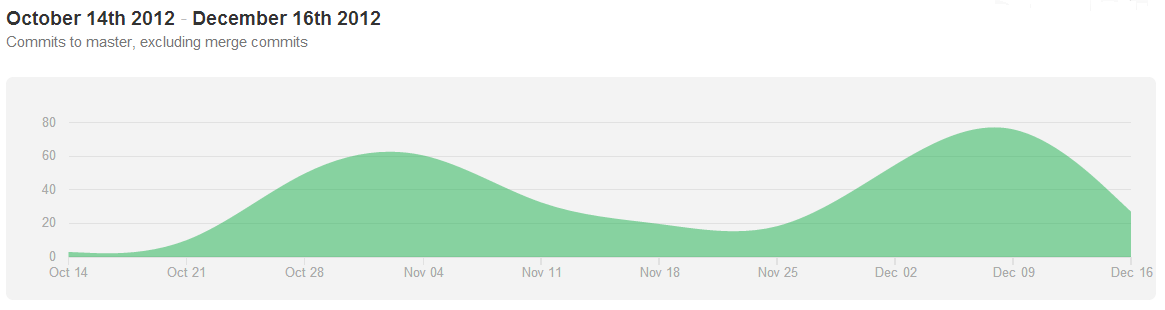
\includegraphics []{Indhold/arbejdsintensitet.png}
\caption {Billedet viser hvor ofte vi har "commitet" nye filer eller nyt arbejde til vores fælles mappe.}
\label {arbejde}
\end{figure}


\end{document}
 %\chapter{}
%	\section{SMS teknologi}
%	Langt de fleste mennesker beskæftiger sig dagligt med SMS'er - dog uden at vide hvad der i virkeligheden sker, når der sendes en SMS. Selv når en mobiltelefon ikke er i brug, sender og modtager den små datapakker til/fra SMS-centeret. Disse data hjælper blandt andet med at lokalisere de basestationer, mobiltelefonen er tættest på.

Når en SMS-besked bliver sendt fra en mobiltelefon, bliver den i første omgang sendt til mobilcentralen via basestationerne. Når mobilcentralen modtager beskeden bliver den overført til et SMS-center (SMSC). SMS-centeret tager sig af at sende beskeden til den rette modtager, ved at overføre den til den ønskede modtagers SMS-center. Når beskeden når frem til den pågældendes center, bliver den, hvis det er muligt, overført til mobilcentralen der sender beskeden til modtageren. SMS-centeret kan endvidere sende en bekræftelse til afsenderen, når beskeden bliver leveret til modtageren. Et overblik over kommunikationen ses i figur \ref{smsTransm}. Alt dette er muligt via Signaling System no. 7 - som er en protokol suite, der indeholder forskellige protokoller. Protokollerne benyttet af SMS-systemer, befinder sig mere specifikt i SS7 suitens Mobile Application Part (MAP). \cite{Pro_1} \cite{sms_max1}

\noindent
\begin{figure}[hba]
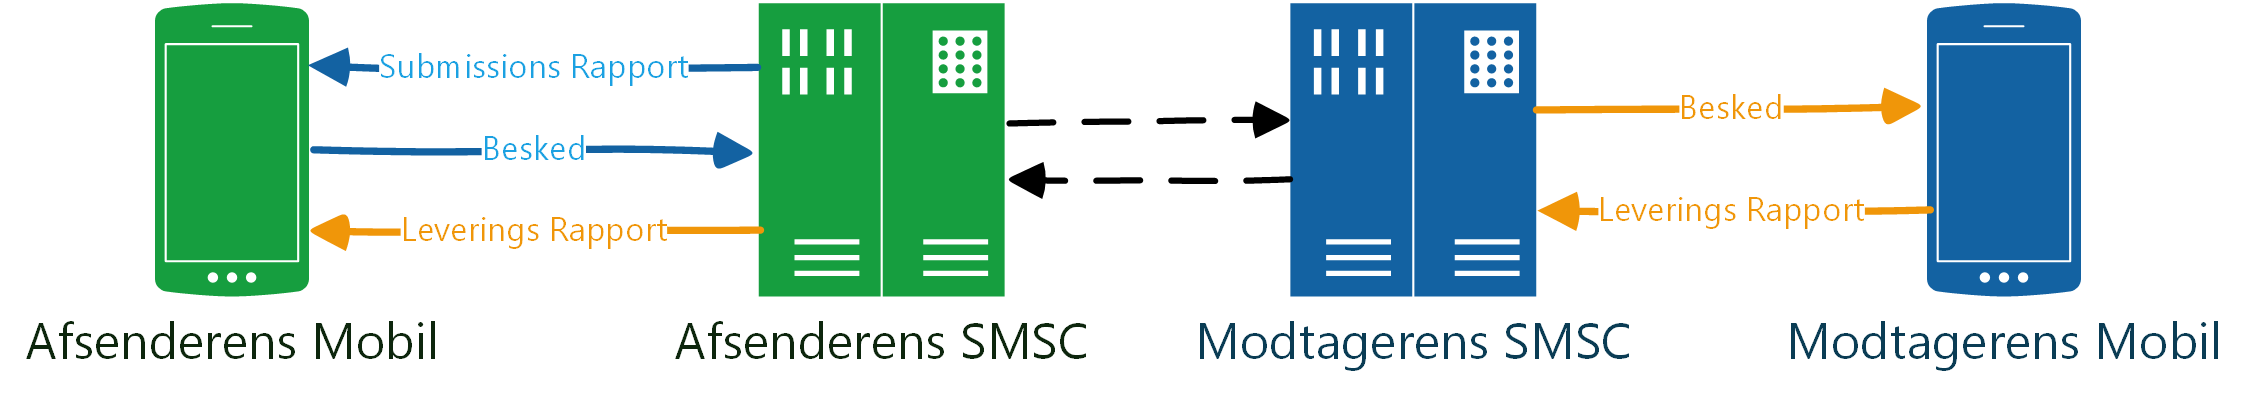
\includegraphics[width=\linewidth]{Billeder/Mobil.png}
\caption {Kommunikationen ved transmission af SMS-beskeder.}
\label{smsTransm}
\end{figure}

Signalerings systemerne i MAP er efter design begrænset til visse størrelser af data. Da man byggede SMS-systemet, talte man tegnene i forskellige beskeder, hvorefter man fandt ud af, at langt de fleste var under 160 tegn. Man mente derfor, at 160 tegn var rigeligt til at rumme de fleste beskeder, hvorved en SMS-beskeds maksimale størrelse blev derfor defineret til 160 tegn. Efter introduktion af udvidede tegnsæt er definitionen præciseret til 1120 bits (160 tegn * 7 bit). \cite{sms_max1} \cite{sms_max2}


Da begrænsningen er defineret i bits, er beskedens maksimale længde afhængig af det anvendte tegnsæt. Det mest almindelige tegnsæt er det grundlæggende 7-bit GSM alfabet. Dette alfabet benytter 7-bits til at symbolisere tegn, hvilket udgør 128 forskellige muligheder. 7-bit GSM alfabetet begrænser derfor en SMS-beskeds længde til 1120/7 bits = 160 tegn. Når der er brug for mere avancerede specialtegn, bruger SMS-systemer UCS-2 tegnsættet. Dette tegnsæt benytter 2 okteter - altså 16 bits - til repræsentation af ét tegn. Ved brug af dette tegnsæt mindskes den maksimale længde derfor ned til 1120/16 = 70 tegn. \cite{sms_pdu}

Enhver SMS-besked indeholder også en header\cite{sms_pdu}, som der er afsat plads til udover de 140 okteter. En SMS-header indeholder typisk data som f.eks. afsenderens telefonnummer, længden af beskeden, benyttet tegnsæt og lignende. Hvis en SMS-besked bliver længere end grænsen, på det benyttede tegnsæt, bliver beskeden delt op i flere beskeder. Når en besked bliver delt op, skrives der information til fletning af beskeden i headeren - og da der ikke er afsat plads til ekstra header information, bliver der brugt 6 okteter af de oprindelige 140 i beskeden. Dette begrænser længden yderligere til 153 ved 7-bit encoding og 67 ved 16-bit encoding. 
